\subsection{Model \textit{Use case}}
Dari beberapa kebutuhan fungsional serta karakteristik pengguna, dapat dibuat \textit{use case} yang mengelompokan serta menggambarkan relasi antara aktor dan aksi yang dapat dilakukan. Use case akan memiliki identifikasi yang berawalan dengan UC diikuti oleh dua angka. Use case secara jelas dituliskan pada tabel dibawah ini.

\begin{table}[h]
  \caption{Tabel Use case}
  \label{tab:penjelasan-usecase-diagram}
  \centering
  \begin{tabular}{|c|p{4cm}|p{8cm}|}
    \hline
    ID   & Use case                                   & Deskripsi                                                                                                                                  \\
    \hline
    UC01 & Mendaftarkan perusahaan                    & Sistem memberikan akses kepada admin untuk mendaftarkan perusahaan yang ingin mendaftar ke dalam sistem                                    \\
    \hline
    UC02 & Mendaftarkan \textit{user}                 & Sistem memberikan akses kepada admin untuk mendaftarkan \textit{user} ke perusahaan tertentu                                               \\
    \hline
    UC03 & Manajemen perusahaan                       & Sistem memberikan akses kepada admin untuk melakukan manajemen terhadap seluruh perusahaan yang terdaftar pada sistem                      \\
    \hline
    UC04 & Manajemen \textit{user}                    & Sistem memberikan akses kepada admin untuk melakukan manajemen terhadap seluruh \textit{user} yang terdaftar pada sistem                   \\
    \hline
    UC05 & Login                                      & Sistem memberikan akses kepada \textit{user}                                                                                               \\
    \hline
    UC06 & Melihat detail perusahaan                  & Sistem memberikan akses kepada \textit{user} untuk melihat perusahaanya                                                                    \\
    \hline
    UC07 & Melihat \textit{user} pada satu perusahaan & Sistem memberikan akses kepada \textit{user} user lainnya pada satu perusahaan                                                             \\

    \hline
    UC08 & Manajemen \textit{perangkat}               & Sistem memberikan akses kepada \textit{user} untuk melihat, membuat, serta menghapus \textit{perangkat} yang terdaftar pada sistem         \\
    \hline
    UC09 & Manajemen \textit{groups}                  & Sistem memberikan akses kepada \textit{user} untuk melihat, membuat, serta menghapus \textit{groups} yang terdaftar pada sistem            \\
    \hline
    UC10 & Manajemen \textit{deployment images}       & Sistem memberikan akses kepada \textit{user} untuk melihat, membuat, serta menghapus \textit{deployment images} yang terdaftar pada sistem \\
    \hline
    UC11 & Manajemen \textit{deployment plan}         & Sistem memberikan akses kepada \textit{user} untuk melihat, membuat, serta menghapus \textit{deployment plan} yang terdaftar pada sistem   \\
    \hline
    UC12 & Melakukan \textit{Remote deployment}       & Sistem memberikan akses kepada \textit{user} untuk melakukan \textit{deployment} kepada target perangakt ataupun \textit{groups}           \\
    \hline
    UC13 & Melihat riwayat \textit{deployment}        & Sistem memberikan akses kepada \textit{user} untuk melihat riwayat \textit{deployment} yang telah dilakukan                                \\
    \hline
  \end{tabular}
\end{table}

Dari pemetaan \textit{Use case} pada \textbf{tabel \ref{tab:penjelasan-usecase-diagram}}, dapat dibuat sebuah diagram yang menghubungkan relasi antara aktor dengan usecasenya. Relasi  aktor dengan kapabilitas fungsional sistem dapat dilihat pada diagram use case berikut.

\begin{figure}[h]
  \centering
  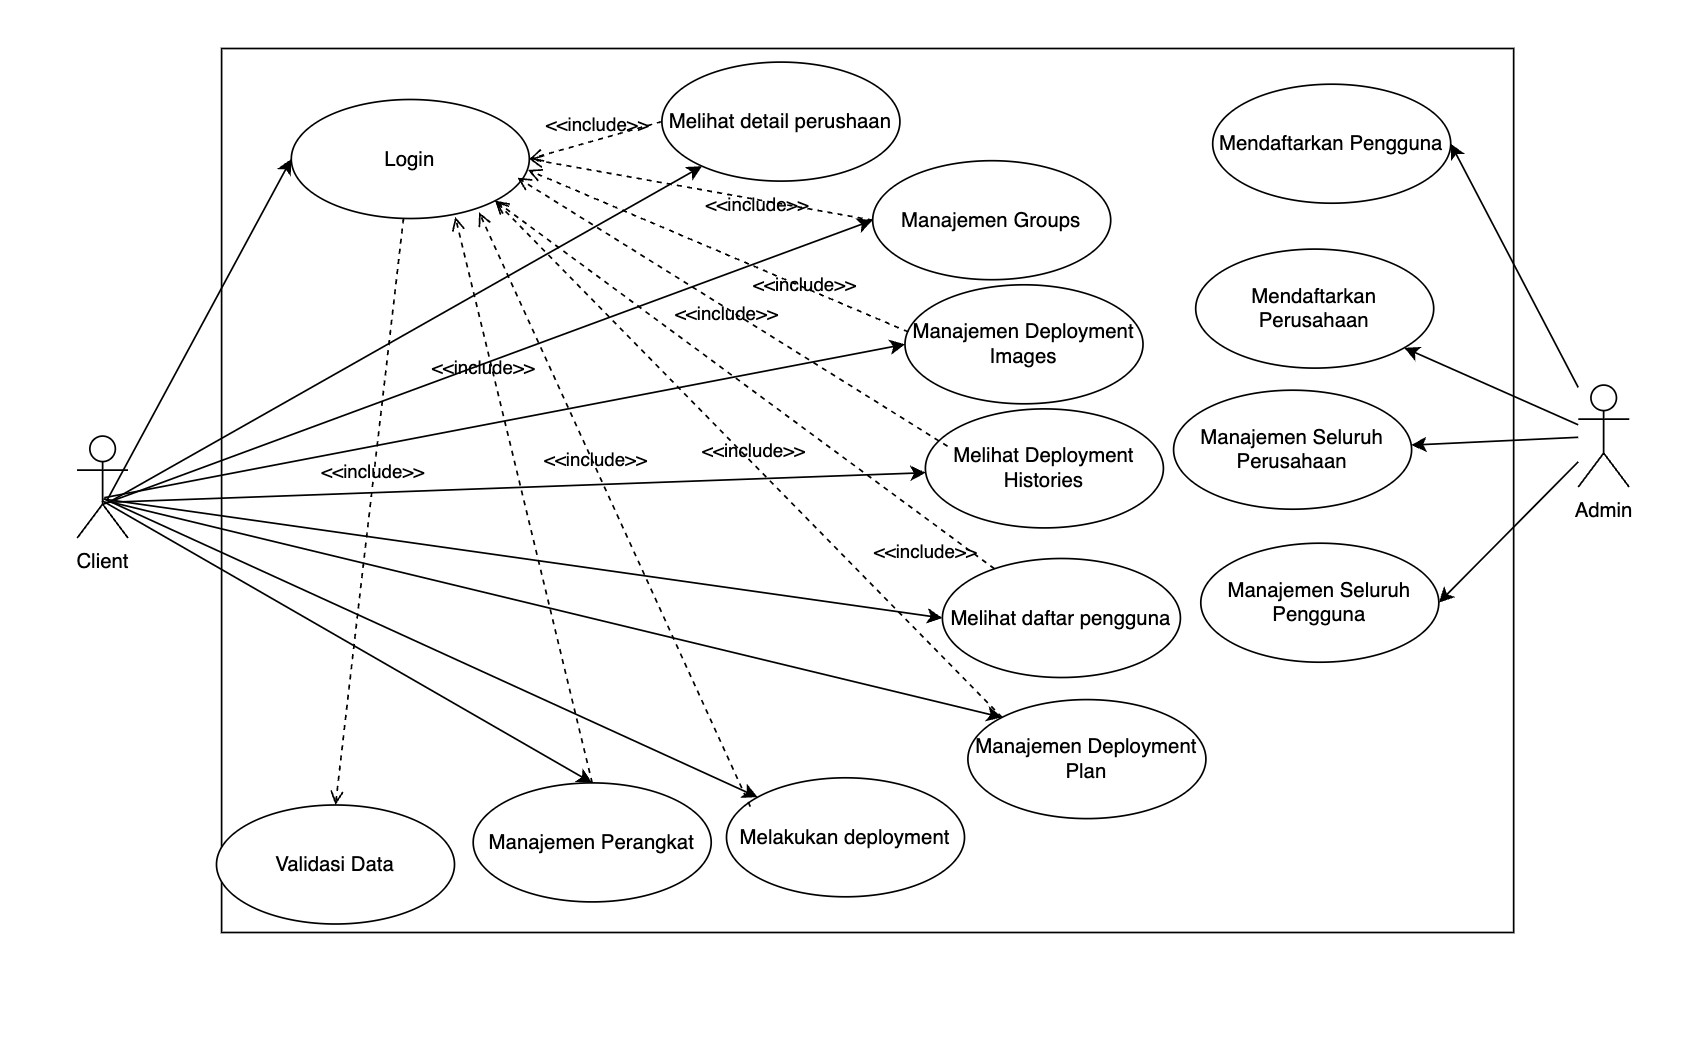
\includegraphics[width=1\textwidth]{resources/chapter-3/usecase-diagram.jpg}
  \caption{Usecase Diagram}
  \label{fig:usecase-diagram}
\end{figure}